%%%%%%%%%%%%%%%%%%%%%%%%%%%%%%%%%%%%%%%%%%%%%%%%%%%
%
%  New template code for TAMU Theses and Dissertations starting Fall 2012.  
%  For more info about this template or the 
%  TAMU LaTeX User's Group, see http://www.howdy.me/.
%
%  Author: Wendy Lynn Turner 
%	 Version 1.0 
%  Last updated 8/5/2012
%
%%%%%%%%%%%%%%%%%%%%%%%%%%%%%%%%%%%%%%%%%%%%%%%%%%%

%%%%%%%%%%%%%%%%%%%%%%%%%%%%%%%%%%%%%%%%%%%%%%%%%%%%%%%%%%%%%%%%%%%%%%
%%                           SECTION III
%%%%%%%%%%%%%%%%%%%%%%%%%%%%%%%%%%%%%%%%%%%%%%%%%%%%%%%%%%%%%%%%%%%%%
%%%%%%%%%%%%%%%%%%%%%%%%%%%%%%%%%%%%%%%%%%%%%%%%%%%
%%%%%%%%%%%%%%%%%%%%%%%%%%%%%%%%%%%%%%%%%%%%%%%%%%%
\chapter{\uppercase {Application of the entropy viscosity method to the multi-D Burger's equation}}\label{chap:burger_chap3}
%%%%%%%%%%%%%%%%%%%%%%%%%%%%%%%%%%%%%%%%%%%%%%%%%%%
%%%%%%%%%%%%%%%%%%%%%%%%%%%%%%%%%%%%%%%%%%%%%%%%%%%
The multi-D Burger's equation is solved using the entropy viscosity method described in \sect{sec:evm_hyp_sc_sct1b}. The equation with the viscous regularization and the definition of the viscosity coefficients are recalled, and the treatment of the boundary condition in also explained in \sect{sec:burger_sct2b}. 1- and 2-D numerical results are presented in \sect{sec:num_sct2b}. The objective of this section is to present numerical results obtained with the entropy viscosity method for the simple hyperbolic scalar Burger's equation before dealing with hyperbolic system of equations. The multi-physics framework MOOSE \cite{Moose} was used to implement the multi-D Burger's equation. The code name is Badger.

%==============================================================================
\section{The multi-D Burger's equation}\label{sec:burger_sct2b}
%==============================================================================
We recall the multi-D Burger's equation (\eqt{eq:burger_eq_sct2b}) with the viscous regularization and the definition of the viscosity coefficient (\eqt{eq:burger_visc_sct2b}).
%
\begin{subequations}\label{eq:burger_sct2b}
%
\begin{equation}\label{eq:burger_eq_sct2b}
\partial_t u(\vec{r},t) + \div \left( \frac{u(\vec{r},t)^2}{2} \vec{n} \right) = \div \left( \mu(\vec{r},t) \grad u(\vec{r},t) \right)
\end{equation}
%
\begin{equation}\label{eq:burger_visc_sct2b}
\left\{
\begin{array}{l}
\mu(\vec{r},t) = \min \left( \mu_{max} (\vec{r},t),  \mu_e(\vec{r},t)\right) \\
\mu_{max} (\vec{r},t) = \frac{h}{2} | u(\vec{r},t) | \\
\mu_e(\vec{r},t) = h^2 \frac{\max\left( R_e(\vec{r},t), J \right)}{|| s(\vec{r},t) - \bar{s}(t) ||_\infty}
\end{array}
\right.
\end{equation}
%
\begin{equation}\label{eq:burger_res_sct2b}
\left\{
\begin{array}{l}
R_e(\vec{r},t) = \partial_t s(\vec{r},t) + \grad \left( u(\vec{r},t) s(\vec{r},t) \right) \\
J = \left[ u(\vec{r},t) s(\vec{r},t) \right]
\end{array}
\right.
\end{equation}
%
\end{subequations}
%
where $\vec{n}$ is a vector whom definition depends on the dimension of the domain: $\vec{n} = \left(1, 0, 0 \right)$ in 1-D, $\vec{n} = \left(1, 1, 0 \right)$ in $2$-D and $\vec{n} = \left(1, 1, 1 \right)$ in $3$-D. The entropy function is denoted by $\eta$ and is taken equal to the convex function $\eta(\vec{r},t) = u(\vec{r},t)^2/2$ for the two examples presented in \sect{sec:num_sct2b}. The continuous Galerkin finite element method described in \chap{chap:disc_chap2} along with the second-order temporal integrator BDF2 are used to discretize \eqt{eq:burger_eq_sct2b}. Such discretization requires to compute the flux at the boundary of the computational domain \eqt{en:va_system_weak5}. Our implementation of the boundary condition for Burger's equation is based on the sign of the dot product $u(\vec{r},t) \vec{n} \cdot \hat{n} $ at the boundary, where $\hat{n}$ is the outward normal to the boundary. For Burger's equation it was demonstrated in \sect{sec:mat_ppr_sct1b} that the eigenvalue is the solution itself $\lambda = u$. Being at the boundary, two cases have to be distinguished: 
\begin{itemize}
\item $u(\vec{r},t) $ is negative: the wave enters the computational domain and thus, information needs to be supplied to the code. This boundary condition can be enforced either weakly or strongly. In the former case, the boundary value is specified in the input file, for instance, and used to compute the flux at the boundary. In the later case, the boundary value is still specified but strongly enforced with a Dirichlet boundary condition. This approach is valid for both implicit and explicit temporal integrators.
\item $u(\vec{r},t) $ is positive: the wave exits the computational domain. The flux is computed with the value of the solution from the last Krylov iteration supplied by the temporal implicit solver. Because of the iterative process, the information normally carried by the waves is transmitted to the boundary. This approach is only valid with an implicit solver. When using an explicit solver, the solution at the new time on the boundary is obtained from the characteristic equation that is integrated over the first cell in.
\end{itemize}
\textcolor{red}{can you say a few words about the incoming and outgoing waves WHEN explicit time integration is used, for completeness} \tcb{done}
% The above method for is a-dimensional and was used to obtain the numerical results presented in \eqt{sec:num_sct2b}.

%==============================================================================
\section{Numerical results}\label{sec:num_sct2b}
%==============================================================================
Two typical numerical tests are presented in order to illustrate the main features of the entropy viscosity method when applied to the multi-D Burger's equation.
%------------------------------------------------------------------------------------------------------
\subsection{1-D numerical result}\label{sec:1dnum_sct2b}
%------------------------------------------------------------------------------------------------------
We consider a 1-D computational domain of length $L=1$ $m$ discretized by an uniform mesh of $100$ elements. The initial condition consists of a smooth sinusoidal function $u(x,0) = \sin \left( 2 \pi x \right)$. The values at the left and right boundaries are set to zero and enforced by Dirichlet conditions. The numerical solution is run until $t=0.2$ $s$ with a $CFL$ of one. In order to investigate the effect of the entropy viscosity method onto the numerical solution, three tests are performed. In the first test, the numerical solution is run with first-order viscosity coefficient which implies $\mu(x,t) = \mu_{max}(x,t)$ at all point of the computational domain and for all time. Then, the same run is performed using the definition of $\mu(x,t)$ recalled in \eqt{eq:burger_visc_sct2b}. Lastly, the code is run without stabilization, $\mu(x,t) = 0$. The objective of running these three cases is to demonstrate the usefulness of the stabilization method and also to show the gain in accuracy when a high-order stabilization method is utilized. Numerical results are shown in \fig{fig:1d_burger_free} through \fig{fig:1d_burger_visc}. 
%
\begin{figure}[H]
        \centering
        \begin{subfigure}[b]{0.495\textwidth}
                \centering
                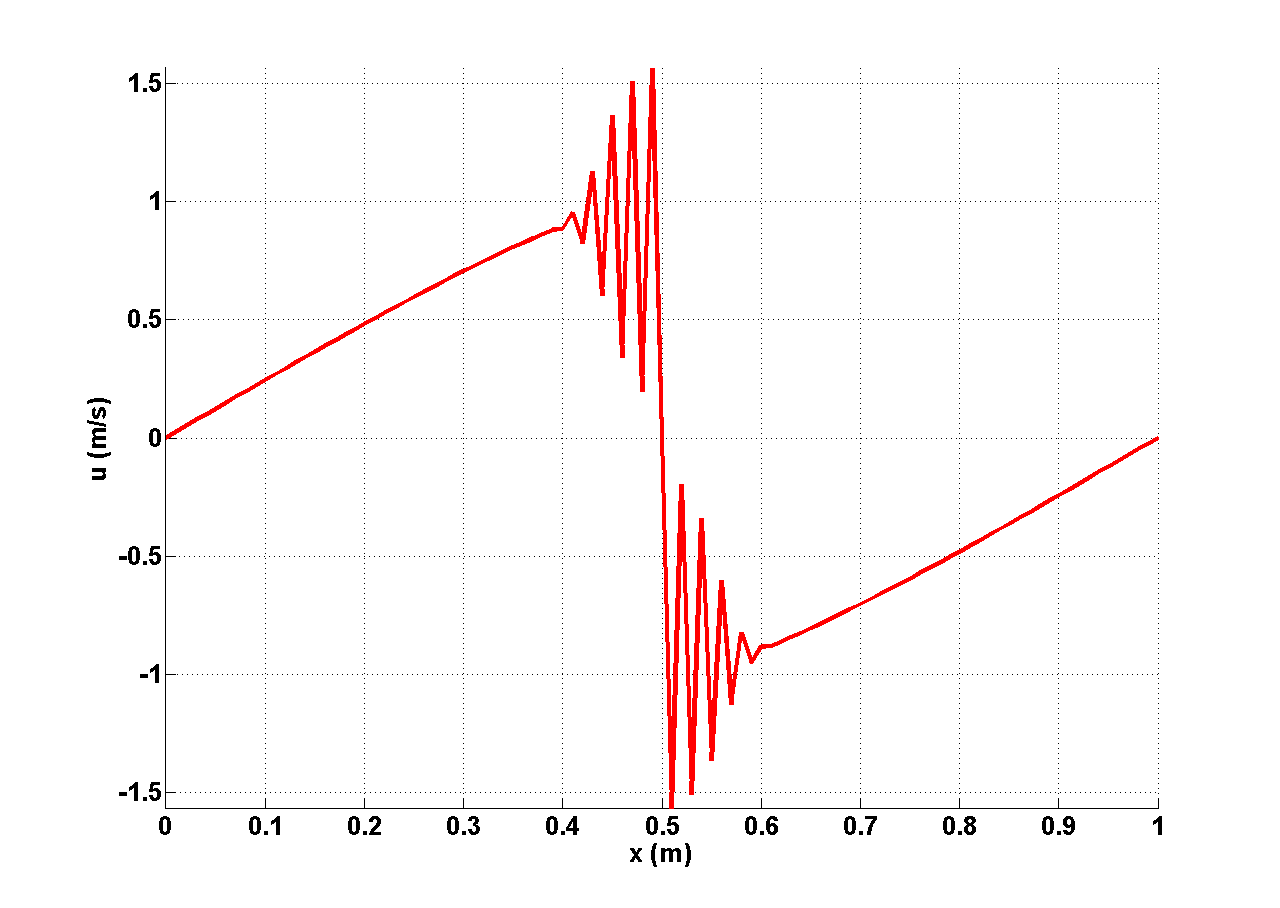
\includegraphics[width=\textwidth]{figures/1D_sol_free.png}
                \caption{Solution profile without stabilization.}
                \label{fig:1d_burger_free}
        \end{subfigure}%
%
        \begin{subfigure}[b]{0.495\textwidth}
                \centering
                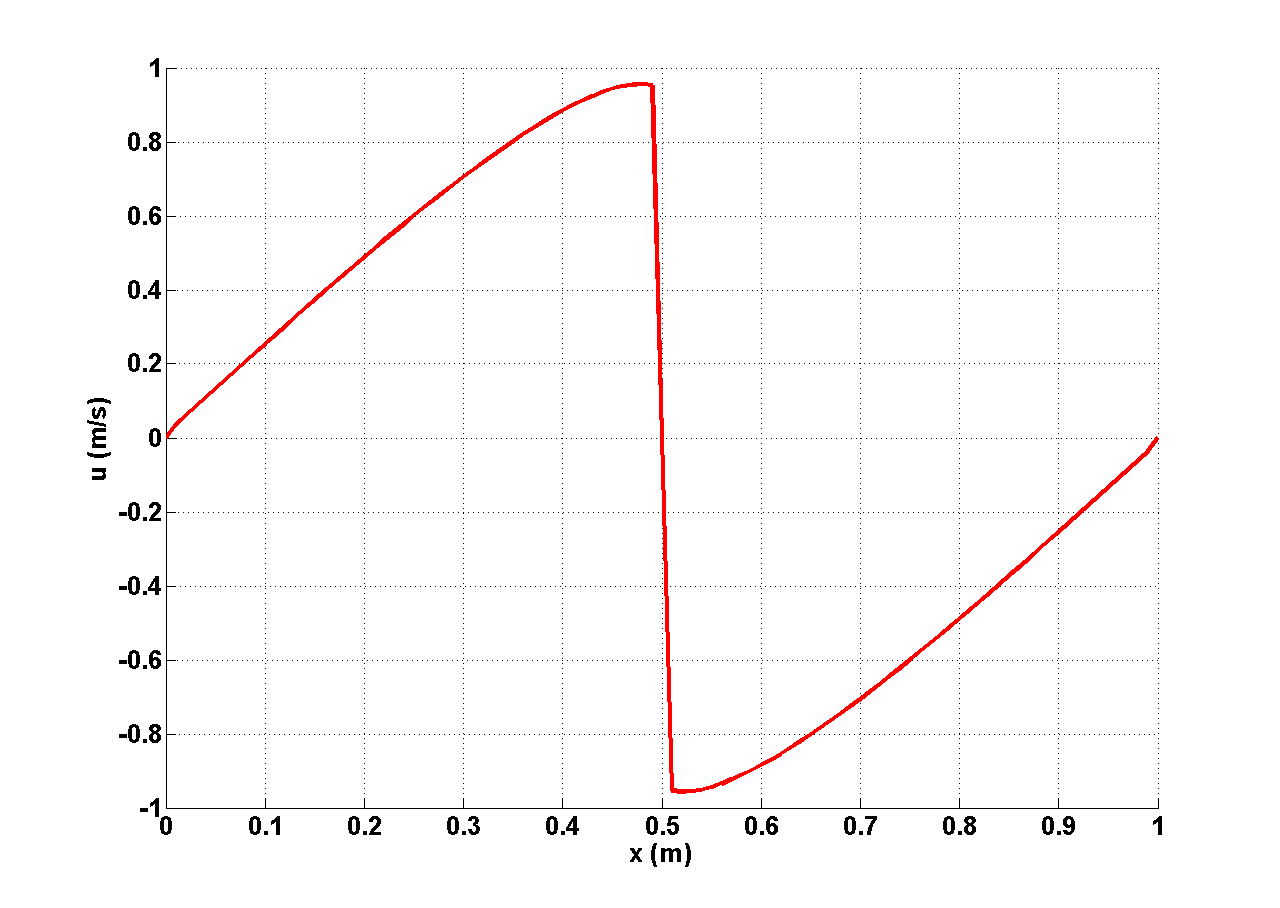
\includegraphics[width=\textwidth]{figures/1D_sol_fo.png}
                \caption{Solution profile with first-order viscosity.}
                \label{fig:1d_burger_fo}
        \end{subfigure}
        
        \begin{subfigure}[b]{0.495\textwidth}
                \centering
                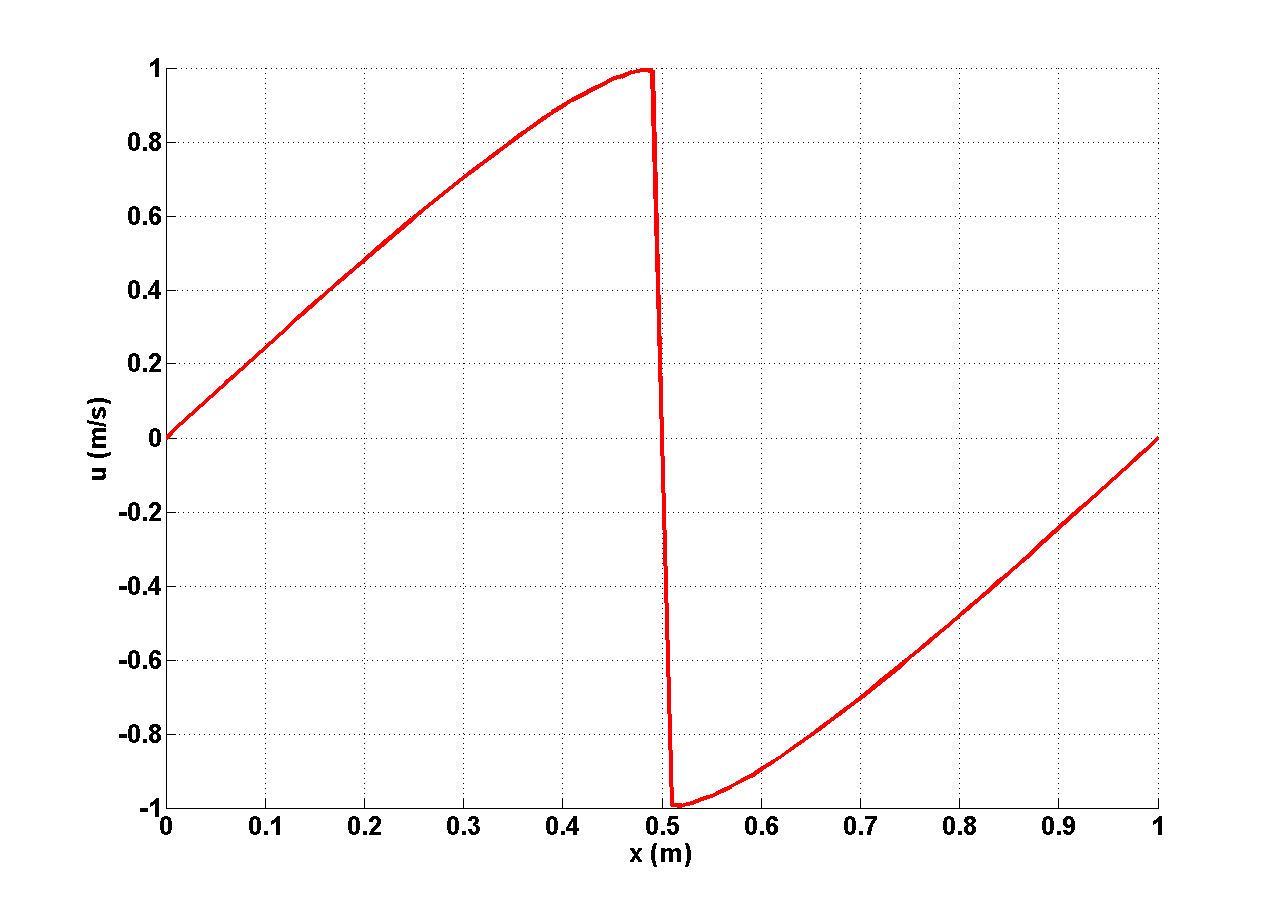
\includegraphics[width=\textwidth]{figures/1D_sol_ev.png}
                \caption{Solution profile with the EVM.}
                \label{fig:1d_burger_ev}
        \end{subfigure}
%       
        \begin{subfigure}[b]{0.495\textwidth}
                \centering
                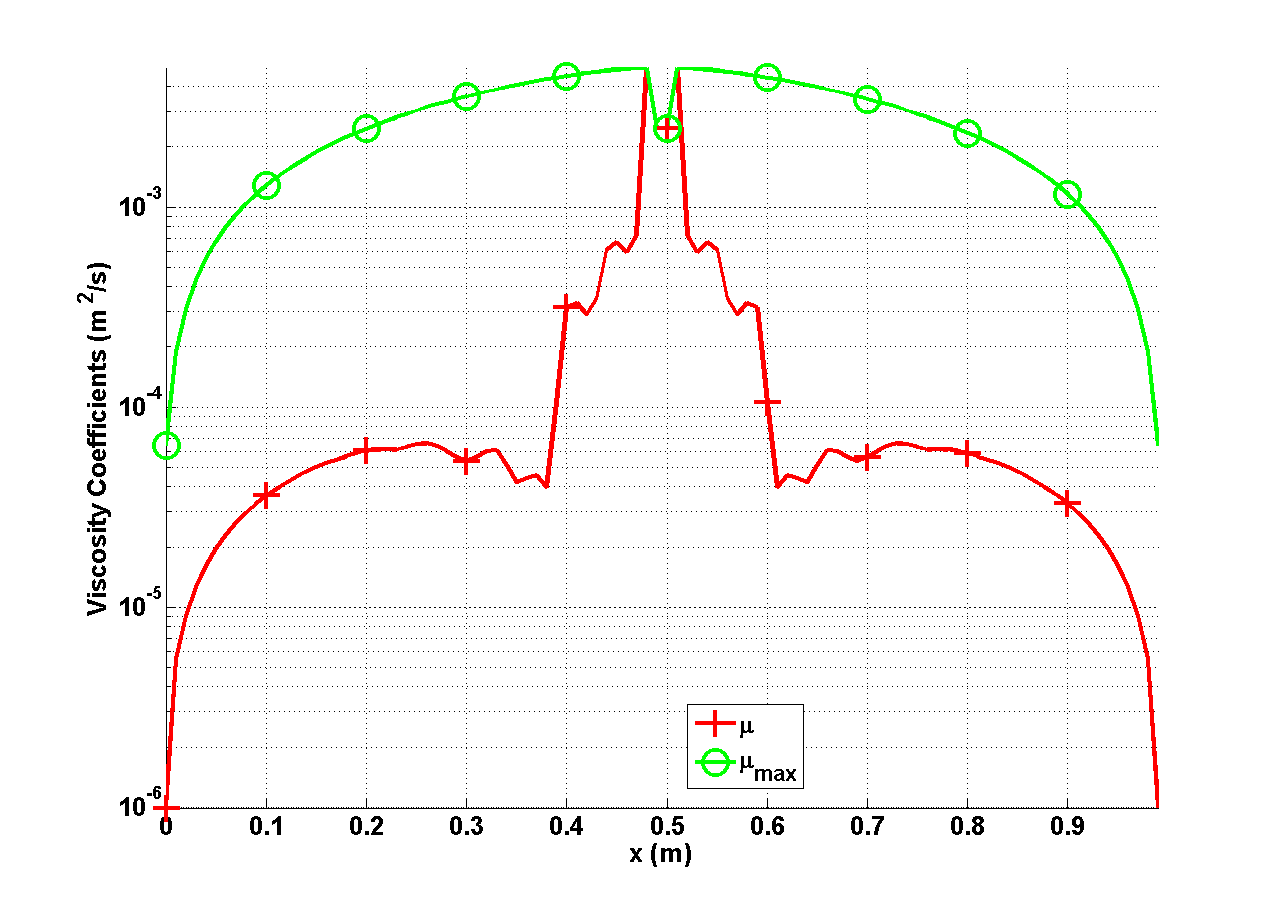
\includegraphics[width=\textwidth]{figures/1D_visc.png}
                \caption{Viscosity coefficient profiles.}
                \label{fig:1d_burger_visc}
        \end{subfigure}
\end{figure}
%
In \fig{fig:1d_burger_free}, no stabilization  is used and numerical instabilities are observed in the shock region. When run with the over-dissipative first-order viscosity coefficient, the solution does not display any instabilities but the shock amplitude is smoothed as shown in \fig{fig:1d_burger_fo}. Lastly, the numerical solution obtained with the EVM in \fig{fig:1d_burger_ev} is very close to the exact solution: the shock amplitude is preserved and the solution is stable. The viscosity coefficients are shown in \fig{fig:1d_burger_visc} on a log-scale: the high-order viscosity coefficient $\mu_e$ is peaked in the shock region and is small anywhere else. This behavior is expected and corresponds to the theoretical approach detailed in \sect{sec:evm_hyp_sc_sct1b}. It was demonstrated in \cite{valentin} that high-order accuracy is preserved with the EVM when the solution is smooth (i.e. away from the shock region). It is also noticed the difference of order of magnitude between the high- and first-order viscosity coefficients away from the shock region.
%------------------------------------------------------------------------------------------------------
\subsection{2-D Riemann problem}\label{sec:2dnum_sct2b}
%------------------------------------------------------------------------------------------------------
We now consider a typical 2-D benchmark problem known as Riemann problem. The computational domain consists of a $1 \times 1$ square and the following initial conditions are used:
%
\begin{equation}\label{eq:bg_2d_ic_sct2b}
u(\vec{r},0) = u_0 = \left\{
\begin{array}{l}
+0.5 \text{ for } x \leq 0.5 \text{ and } y \leq 0.5 \\
+0.8 \text{ for } x \geq 0.5 \text{ and } y \leq 0.5 \\
-0.2 \text{ for } x \leq 0.5 \text{ and } y \geq 0.5 \\
-1. \text{ for } x \geq 0.5 \text{ and } y \geq 0.5
\end{array}
\nonumber
\right.
\end{equation}
%
An uniform mesh of $100 \times 100$ elements is used. The solution is run until $t=0.5$ $s$ with a $CFL$ of $0.5$. The numerical solution and the viscosity coefficient profiles are plotted at $t=0.2$ and $t=0.5$ $s$. 
%
\begin{figure}[H]
	\centering
	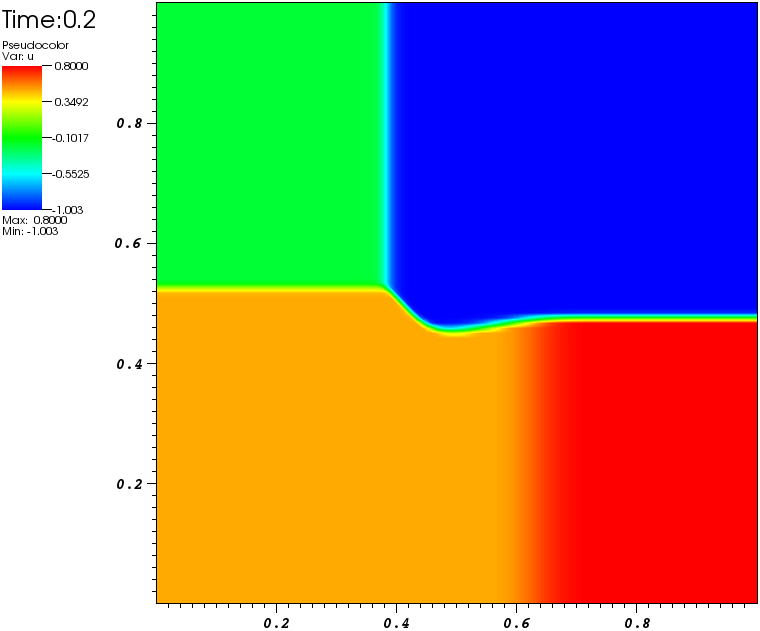
\includegraphics[width=\textwidth]{figures/Burger2D_sol_t0p2.png}
	\caption{Solution profile at $t=0.2$ $s$.}
	\label{fig:2d_burger_sol_t0p2}
\end{figure}
%
\begin{figure}[H]
	\centering
	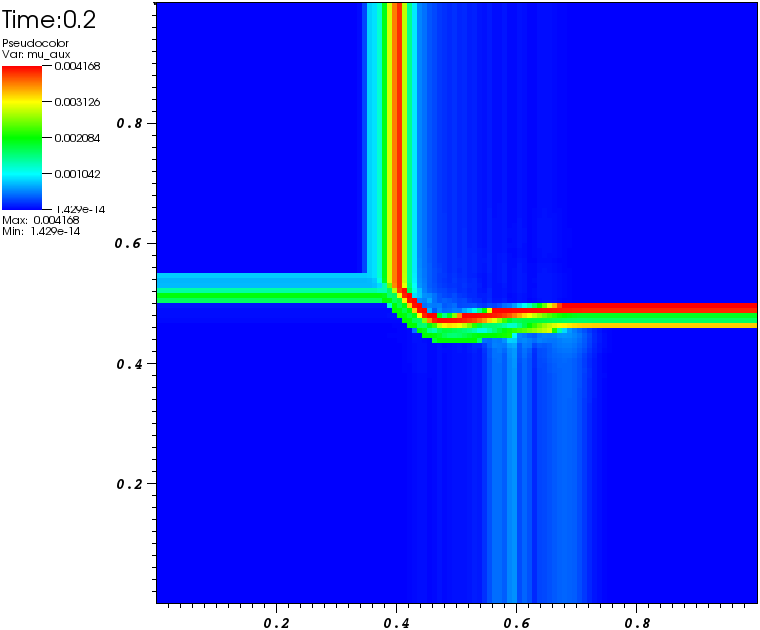
\includegraphics[width=\textwidth]{figures/Burger2D_visc_t0p2.png}
	\caption{Solution profile at $t=0.2$ $s$.}
	\label{fig:2d_burger_visc_t0p2}
\end{figure}
%
\begin{figure}[H]
	\centering
	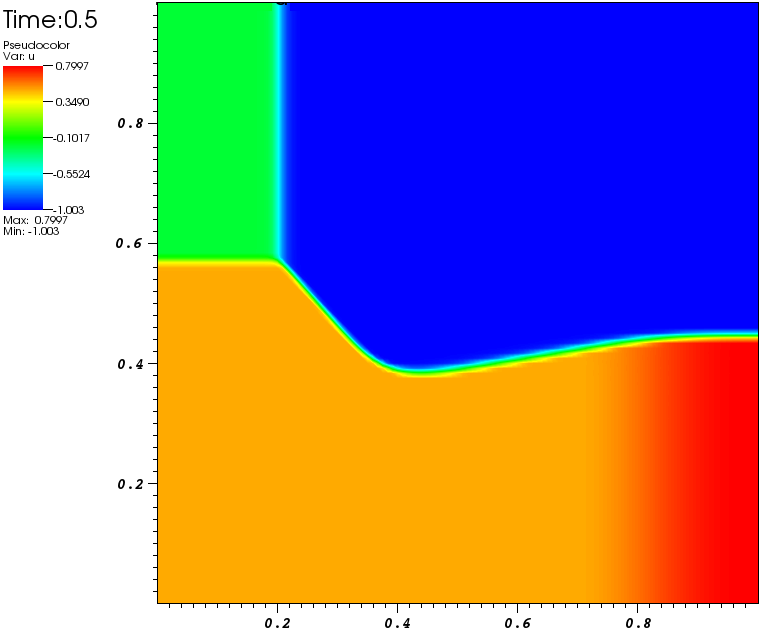
\includegraphics[width=\textwidth]{figures/Burger2D_sol_t0p5.png}
	\caption{Solution profile at $t=0.5$ $s$.}
	\label{fig:2d_burger_sol_t0p5}
\end{figure}
%
\begin{figure}[H]
	\centering
	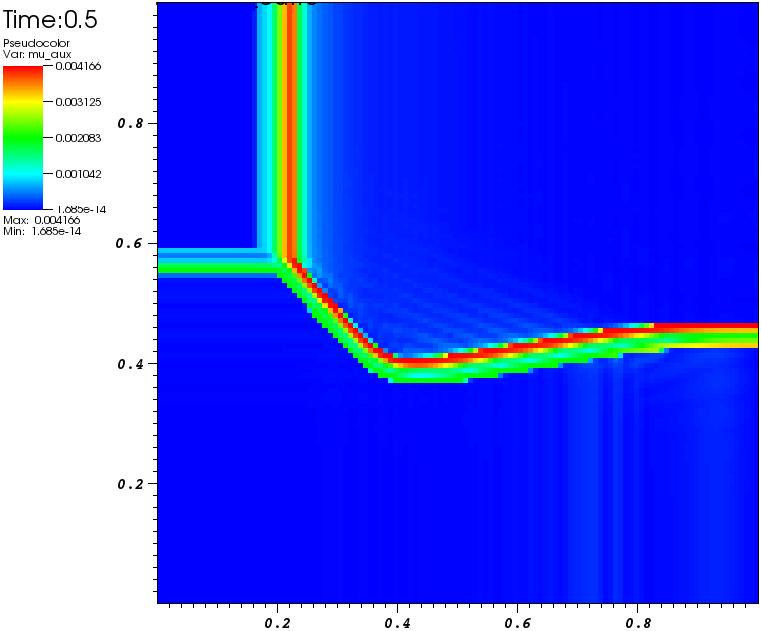
\includegraphics[width=\textwidth]{figures/Burger2D_visc_t0p5.png}
	\caption{Solution profile at $t=0.5$ $s$.}
	\label{fig:2d_burger_visc_t0p5}
\end{figure}
%
The numerical solution is plotted in \fig{fig:2d_burger_sol_t0p2} and \fig{fig:2d_burger_sol_t0p5} at $t=0.2$ and $t=0.5$ $s$, respectively. The numerical solution does not display any oscillations and the shocks are well resolved. The high-order viscosity coefficient is showed in \fig{fig:2d_burger_visc_t0p2} and \fig{fig:2d_burger_visc_t0p5}: the shock is well tracked by the EVM and sufficient dissipation is only added in the shock regions, where saturation to the first-order viscosity is achieved.\\

The above examples were simple illustrations of the capabilities of the EVM when applied to hyperbolic scalar equations. We now focus our attention to the application of the EVM to various hyperbolic systems of equations.